\documentclass[12pt, a4paper, simple]{eskdtext}

\usepackage{_env/gpi_global.env}
\usepackage{_env/gpi_report.env}
\usepackage{_sty/gpi_lst}
\usepackage{_sty/gpi_toc}
\usepackage{_sty/gpi_t}
\usepackage{_sty/gpi_u}

\def \gpiDocTopic {Отчёт лабораторной работы №\gpiDocNum}

\begin{document}
\begin{ESKDtitlePage}
    \ESKDstyle{empty}
    \begin{center}
        \gpiMinEduRep \\
        \gpiEduRep \\
        \gpiKafRep \\
    \end{center}

    \vfill

    \begin{center}
        Тема: <<\gpiTopicRep>>
    \end{center}

    \vfill

    \begin{center}
        \textbf{\gpiDocTopic} \\
        по дисциплине \gpiDisciplineRep \\
    \end{center}

    \vfill

    \begin{flushright}
        \begin{minipage}[t]{7cm}
            Выполнил: \\
            \PageTitleStudentInfo \\
            \hspace{0pt} \\
            Проверил: \\
            \PageTitleTeacherInfo \\
        \end{minipage}
    \end{flushright}

    \vfill

    \begin{center}
        \PageTitleCity~\ESKDtheYear
    \end{center}
\end{ESKDtitlePage}


\ESKDstyle{empty}

\begin{center}
    \textbf{\gpiDocTopic}
\end{center}

\paragraph{} \textbf{Тема}: <<\gpiTopicRep>>

\paragraph{} \textbf{Цель}:
ознакомиться с циклическими алгоритмами и операторами, реализующими эти алгоритмы.
Освоить особенности применения каждого оператора.
Составить программы с использованием всех операторов цикла.

\paragraph{} \textbf{Что нужно сделать}:

\begin{enumerate}
    \item огласно варианту реализовать «Задание 1» в двух версиях:
    одна с применением цикла while, вторая - цикла for.
    Сделать вывод о том, какой вид цикла для данной задачи удобнее применять.
    \item Согласно варианту реализовать «Задание 2» при помощи цикла do-while c условием выхода из цикла.
    Переписать программу при помощи бесконечного цикла do-while (условие которого всегда истина)
    с применением операторов break и continue.
    Сделать вывод, какой вариант программы лучше и почему?
    \item Разработать блок-схемы алгоритмов (2 - по одной на каждую задачу).
\end{enumerate}

При написании программ выполнять проверку всех вводимых значений на возможность использования в программе
(например: если вместо числа введена буква, если вместо положительного n введено отрицательное и т. п.).

\begin{center}
    \textbf{Задание A5}
\end{center}

Написать программу вычисления модулей введенных отрицательных чисел до тех пор,
пока пользователь не введет 0 (для положительных чисел выводить просто сообщение).

\paragraph{} \textbf{Разработка алгоритма}:

Блок-схема на рисунке~\ref{fig:a5}.

\begin{figure}[!h]
    \centering
    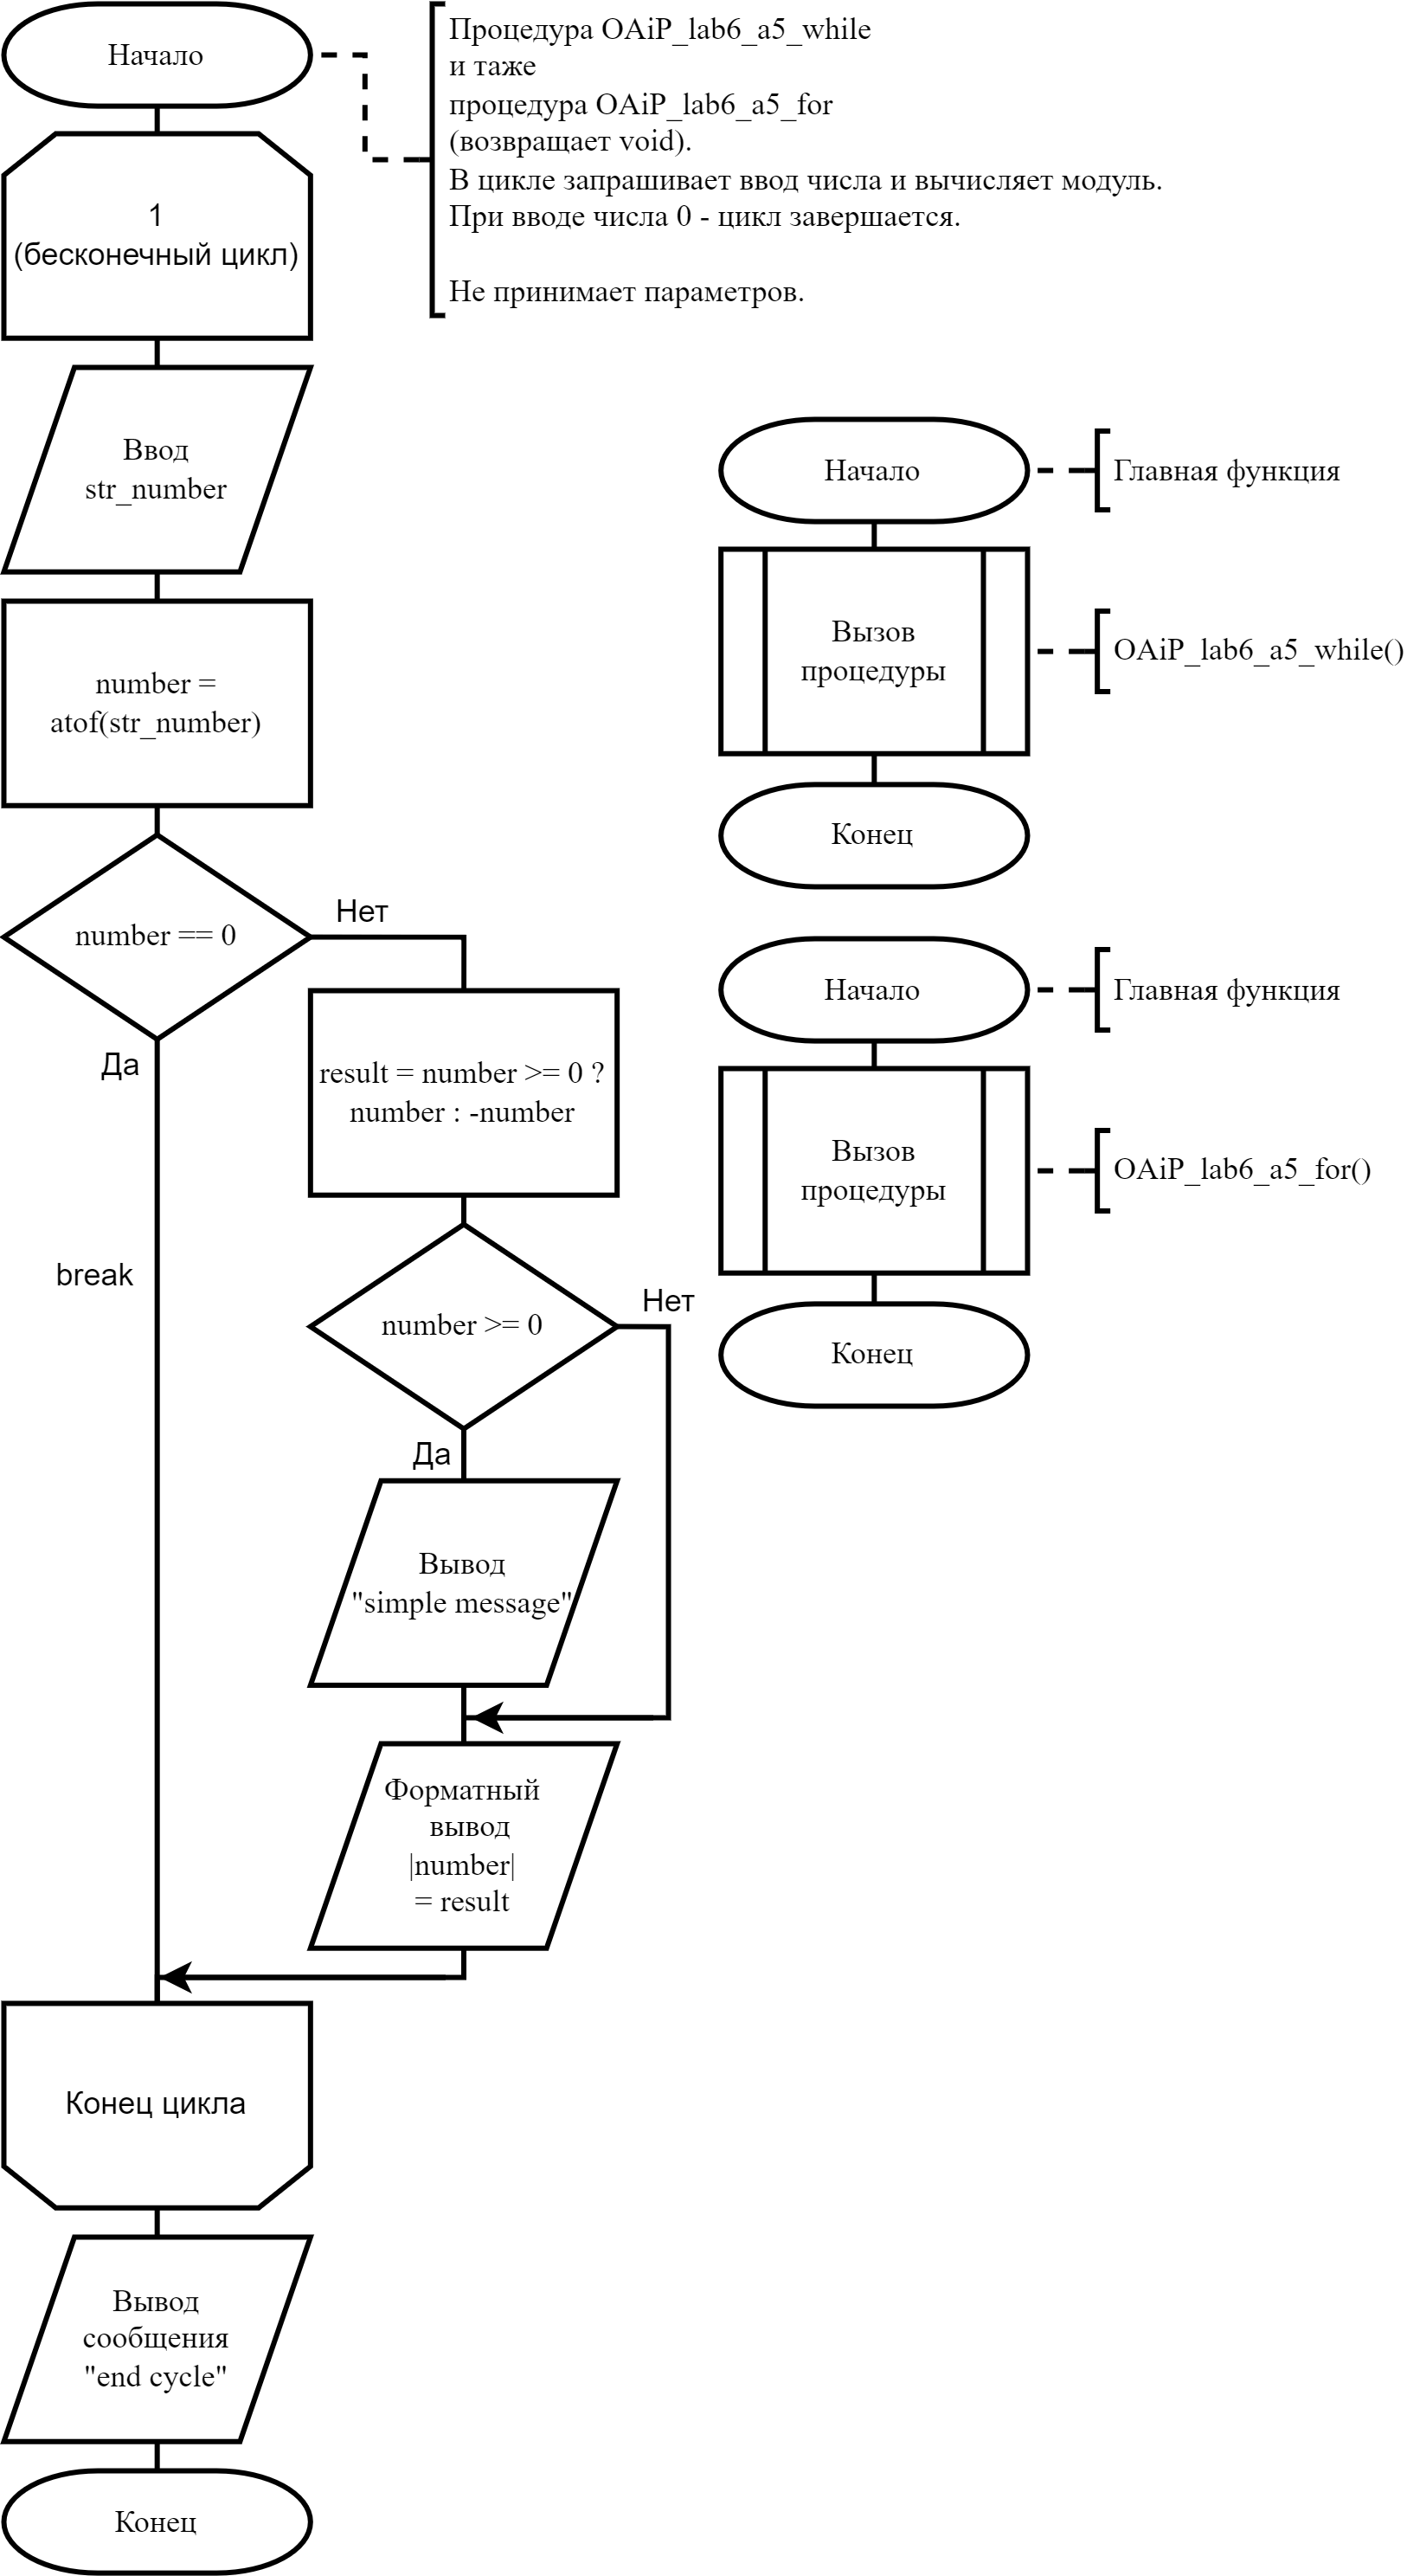
\includegraphics[]
    {../sources/flowcharts/OAiP_lab6_a5.png}
    \caption{Блок-схема}
    \label{fig:a5}
\end{figure}

\paragraph{} \textbf{Исходный код}: 

\lstinputlisting[language=c, name=main.cpp]
{../sources/OAiP_lab6_a5_while/OAiP_lab6_a5_while/main.cpp}

\lstinputlisting[language=c, name=main.cpp]
{../sources/OAiP_lab6_a5_for/OAiP_lab6_a5_for/main.cpp}

\newpage

\begin{lstlisting}[name=Вывод в консоль]
 number: 333
 simple message
 |333.000000| = 333.000000
 
 number: -333
 |-333.000000| = 333.000000 
 
 number: 3.33445566
 simple message
 |3.334456| = 3.334456
 
 number: -3.3456789
 |-3.345679| = 3.345679
 
 number: hello
 end infinity cycle
\end{lstlisting}

\paragraph{} \textbf{Что нужно сделать}:

\begin{center}
    \textbf{Задание Б5}
\end{center}

Вычислить значения функции $f(x)$ на отрезке $[a;b]$ с шагом $h$, кроме $x = a + 2*h$.

$f(x) = cos(x) * e^{-x}$, $[a,b] = [1,2]$, $h = 0.2$

\paragraph{} \textbf{Разработка алгоритма}:

Блок-схема на рисунке~\ref{fig:b5}.

\begin{figure}[!h]
    \centering
    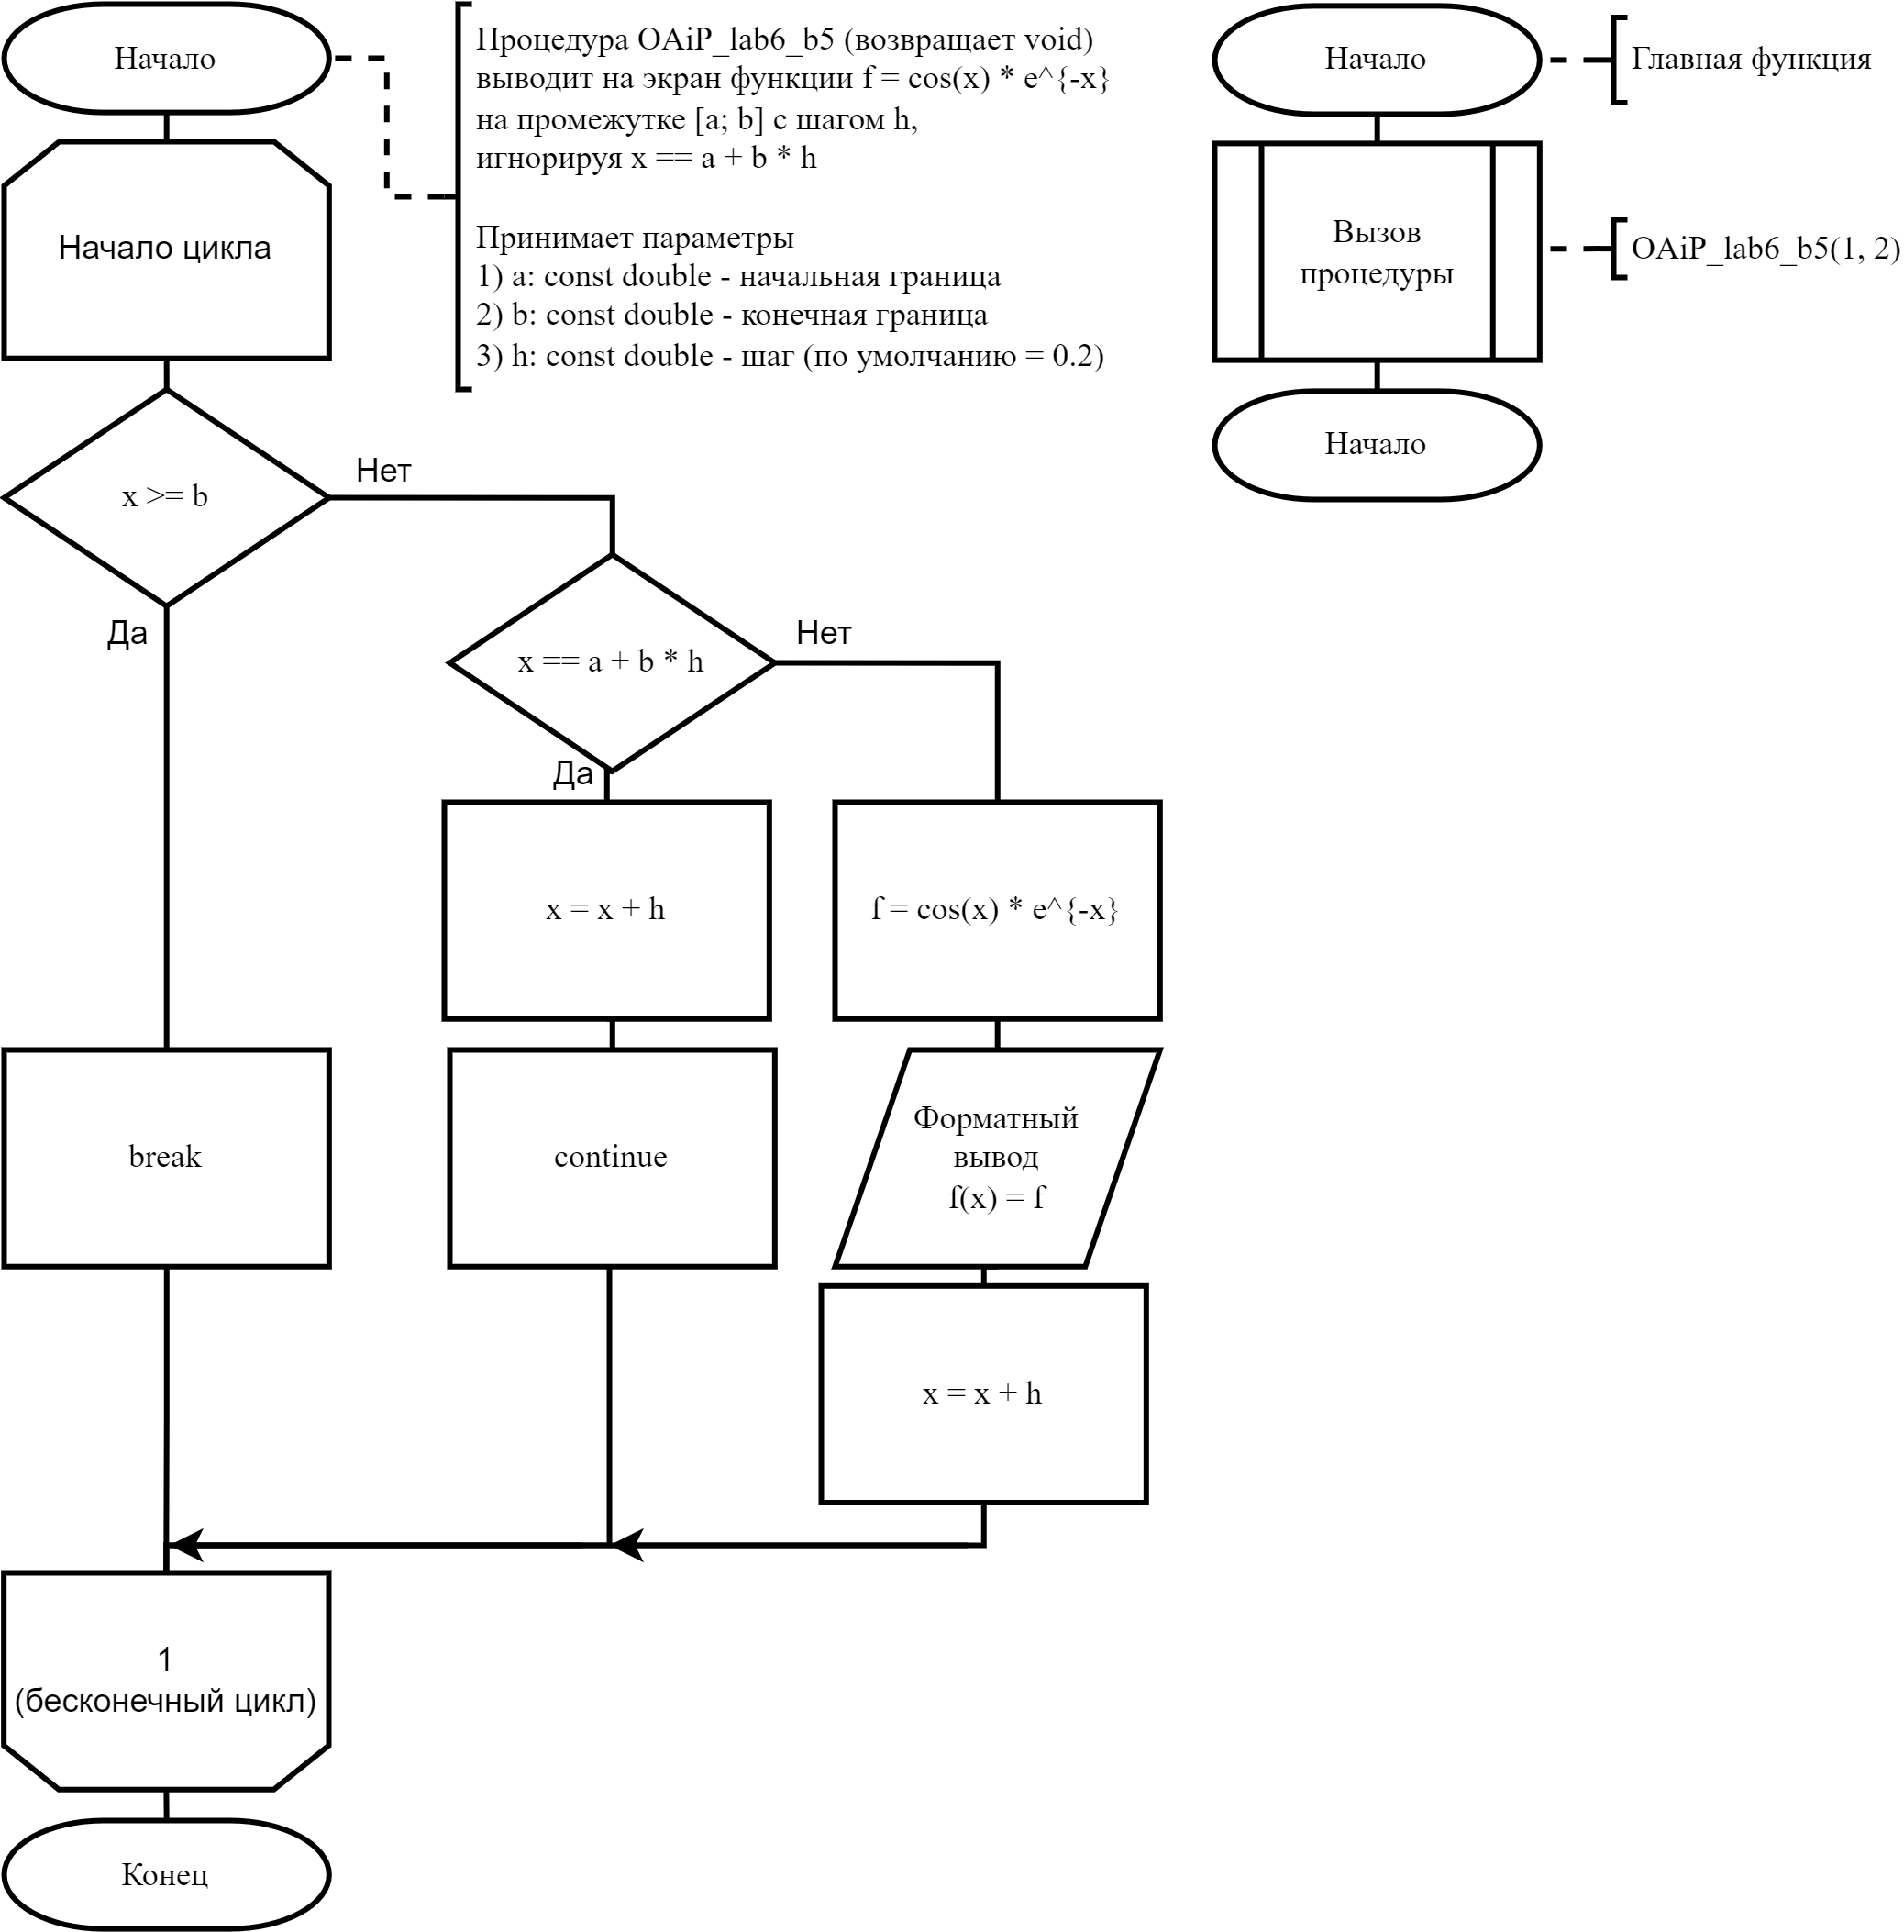
\includegraphics[]
    {../sources/flowcharts/OAiP_lab6_b5.png}
    \caption{Блок-схема}
    \label{fig:b5}
\end{figure}

\paragraph{} \textbf{Исходный код}: 

\lstinputlisting[language=c, name=main.cpp]
{../sources/OAiP_lab6_b5/OAiP_lab6_b5/main.cpp}

\begin{lstlisting}[name=Вывод в консоль]
 f( 1.000000) =  0.198766
 f( 1.200000) =  0.109140
 continue
 f( 1.600000) = -0.005895
 f( 1.800000) = -0.037556
 f( 2.000000) = -0.056319
 break
\end{lstlisting}

\paragraph{} \textbf{Вывод}:
ознакомились с циклическими алгоритмами и операторами, реализующими эти алгоритмы.
Освоили особенности применения каждого оператора.
Составили программы с использованием всех операторов цикла.

% = = = = = = = =
\newpage
% \addcontentsline{toc}{section}{Список использованных источников}
% \section*{Список использованных источников}
\paragraph{} \textbf{Список использованных источников}:
\begin{enumerate}
    \item[1.] Коллекция eskdx v0.98 - eskdx.pdf
    [Электронный ресурс].
    Режим доступа: \url{http://tug.ctan.org/macros/latex/contrib/eskdx/manual/eskdx.pdf}.
    Дата доступа: 30.05.2022.

    \item[2.] Использование системы верстки LaTeX - EVMiS\_Latex.pdf
    [Электронный ресурс].
    Режим доступа: \url{https://www.bstu.by/uploads/attachments/metodichki/kafedri/EVMiS_Latex.pdf}.
    Дата доступа: 30.05.2022.

    \item[3.] Опции пакета hyperref
    [Электронный ресурс].
    Режим доступа: \url{https://grammarware.net/text/syutkin/hyperref_options.pdf}.
    Дата~доступа:~20.02.2022.

    \item[4.] Developers - Docker
    [Electronic resource].
    Mode of access: \url{https://www.docker.com/get-started/}.
    Date~of~access:~04.06.2022.

    \item[5.] Manual installation steps for older versions of WSL | Microsoft Docs
    [Electronic resource].
    Mode of access: \url{https://aka.ms/wsl2kernel}.
    Date~of~access:~04.06.2022.

    \item[6.] LaTeX/Source Code Listings - Wikibooks, open books for an open world
    [Electronic resource].
    Mode of access: \url{https://en.wikibooks.org/wiki/LaTeX/Source_Code_Listings}.
    Date~of~access:~04.06.2022.

    \item[7.] 1sem\_OAiP/OAiP\_lab6.pdf at galanin · BrSTU-PO4-Galanin/1sem\_OAiP
    [Электронный ресурс].
    Режим доступа: \url{https://github.com/BrSTU-PO4-Galanin/1sem_OAiP/blob/galanin/docs/lab6/OAiP_lab6.pdf}.
    Дата доступа: 06.06.2022.
\end{enumerate}

\newpage
\end{document}
